\chapter{Hardware}\label{ch:foundation}
\epigraph{For the things we have to learn before we can do them, we learn by doing them.}{--- Aristotle, The Nicomachean Ethics}
\section{Game environment and rules}\label{sec:game_environment}
As mentioned in section~\ref{sec:research_question}, we were interested in understanding phenomena related to player engagement in~\glspl{pirg}. For this we designed a game where a human plays against a mobile adversarial robot, named Robotower 2.0.

The playground consists of a rectangular area of 4m$\times$4m wide. On each corner of the playground, tubes (henceforth called ``towers'') were placed (details in figure~\ref{fig:towers}). Each tower was equipped with a button (which sits on the tower's cap) and four~\glspl{led} that could be progressively turned on, one by one.  Each~\gls{led} required the button to be pressed for 2.5 seconds, meaning that the tower takes about 10 seconds of button push in order to light up all of its four~\glspl{led}.

The~\glspl{led} are supposed to display the progress of the human player in capturing a specific tower. For a given tower, after turning on all~\glspl{led}, it is said that the player had captured it. When a tower is secured, the robot cannot aim at it anymore.
Button pressing time was cumulative and could be distributed on different moments -- that meant that the player would not lose his progress if he stopped pressing the button before the tower is completely captured. 

The game mechanics and winning conditions were simple enough to allow for a large number of individual to play the game. In order to win, the human players must be able to secure all the existing towers without letting a single one be knocked down by the robot. If, at anytime, a tower falls (because of the robot or the player) the game ends and the human player loses. 

The robot was able to move across the entire playground just as the human player could, and it was only constrained by the fact that an already captured tower, or one whose button is currently being pressed by the player, cannot be teared down. As main interaction channel between the two players,\ie robot and human, the human player could block the robot path at any moment by staying in front of it, causing the later to likely change target tower. Therefore, as consequence of the defined rules, while the player was trying to capture a given tower, the robot could try to tear down any other one.

The game definition in itself is not a trivial task and it is, for the case of~\gls{pirg}, constrained also by the characteristics of the robotic platform. Other than playability and fun, safety is also an important aspect and one that impose heavy bounds to the motion of the robot: a too fast  robot would reduce the perception of the robot been safe to play against, thus limiting the natural interaction. Experimentally, we have evaluated that a robot with a maximum linear speed of 1.4 m/sec would be too difficulty to play against. Moreover, for a mobile robot as ours, speed have some negative impact in the robot control itself, due to mechanical phenomena like wheel slippage, manoeuvrability, and navigation issues (localization and obstacle avoidance). Details about the robot platform are given in section~\ref{sec:roboplat}.

In summary, we designed our game such that we could have an environment rich enough to physically engage human players while allowing for the study of adaptive approaches to support engagement. RoboTower 2.0 stimulates player to perform strong cognitive tasks, like: trajectory planning, attention and spatial reasoning and places itself as an interesting environment from which one could test~\gls{ml} approaches. Next we briefly detail the Towers used in the game in term of their properties and operating system.

%TODO ********************************************
%Here is one of the places were the smartness of game design has to be put in evidence. The Game rules should be described before this chapter or at its beginning, otherwise it would be difficult to understand what are the design choices. All the design choices should be functional to the game. Maybe we should call this section (and the figure) not as "hardware" but as "game design", including Rules, HW and Environment.
% EWERTON: ????? but the games rules are already at the beginning of the chapter.
%**************************************************

\subsection{Towers}\label{sec:towers}
Each tower was powered individually, being capable of transmitting its status to the robot at a constant rate. The circuit used the~\href{https://einstronic.com/wp-content/uploads/2017/06/NodeMCU-ESP8266-ESP-12E-Catalogue.pdf}{NodeMCU V3 ESP8266 ESP-12E} WiFi module\footnote{\url{https://goo.gl/TzAjwi} accessed on December 17th, 2018.} (see figure~\ref{fig:tower_electronics}) whose connection was done via a private network. The communication between towers and the robot was supported through~\gls{tcp} using the rosserial\_server\footnote{\url{http://wiki.ros.org/rosserial_server} accessed on December 17th, 2018.} package. A tilt sensor allows for the detection of fallen towers. Appendix~\ref{app:hard_appendix} provides additional hardware details for the towers. 

%TODO Irrelevant here -> As power supply, a $7.4$V LiPo battery was used on each tower as can been seen on figure~\ref{fig:tower_electronics}. The nominal voltage for the boards was $5$V, which is supplied through a voltage regulator. 
% EWERTON: OK.
%TODO Irrelevant here -> A schematic of the circuit developed to detect such event is provided in figure~\ref{fig:tilt_circuit}. <- Figure not found, but also not needed here. Put these details in appendix. If you like you can put there the complete sections with details, and leave here only the relevant aspects.
% EWERTON: OK.

\begin{figure}[h]
  \centering
  \begin{subfigure}[b]{0.3\textwidth}
  	\centering
    \framebox{\parbox{3cm}{\includegraphics[width=3cm, height=4cm]{images/03-foundation/cap1}}}
	\caption{}
	\label{fig:tower_cap_top}
  \end{subfigure}
  ~ 
  \begin{subfigure}[b]{0.3\textwidth}
  	\centering
    \framebox{\parbox{3cm}{\includegraphics[width=3cm, height=4cm]{images/03-foundation/cap2}}}
	\caption{}
	\label{fig:tower_electronics}
  \end{subfigure}
  ~
   \begin{subfigure}[b]{0.3\textwidth}
	  \centering
      \framebox{\parbox{3cm}{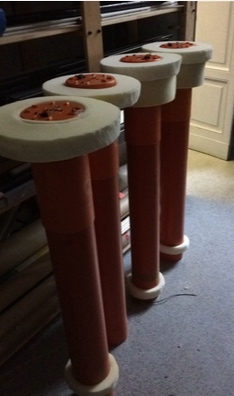
\includegraphics[width=3cm,  height=4cm]{images/04-activity/tubes.jpg}}}
      \caption{}
    \end{subfigure}
  \caption{a) Tower cap containing the button (red square) and~\glspl{led}; b) Tower cap electronics; c) The four towers used in the game (height 110cm).}
  \label{fig:towers}
\end{figure}

\section{The robotic platform}\label{sec:roboplat} 
As depicted in figure~\ref{graph:PIRG_design_structure}, hardware is the core concern for a mobile robot in~\gls{pirg}. In the graph in figure~\ref{graph:HARDWARE_structure} we have detailed some relevant aspects that we considered during our design. The graph is not supposed to give an extensive map of the necessary hardware aspects and their inter relationship, but to instruct the reader on the necessary aspect in this first phase of design taking our development as example. %Naturally, not all mobile robots involved in~\glspl{pirg} will take into account all such concerns. In fact, the original RoboTower~\citep{bonarini_timing_2014} and Jedi Trainer 3.0~\citep{martinoia_physically_2013} were examples of mobile robots that did not considered, for instance, navigation techniques, such as~\gls{slam} and~\gls{oa} and had no sophisticated structural and sensing requirements given the little computing power available.
% EWERTON: OK. But, it is necessary to note that the pigs developed previously were much less complex than our.

Our wheeled robot, called Triskar, had holonomic kinematics,\ie it was free to move in any direction at a speed comparable to that of people in indoor environments (up to 1.4~m/sec). The base consisted of a metallic, triangular-shaped structure where motors, batteries, computer and necessary electronics are embedded. In total, the robot weights $22.3$ kg. Triskar has simultaneously and independently controlled rotational and translational motion capabilities thanks to three omnidirectional wheels actuated by a motor each. The robot's movement on flat floor is as free as the human one, which made it a good base for adversarial~\glspl{pirg} and, in particular, the one that we had designed. 

\begin{figure}[H]
    \centering
    \begin{tikzpicture}[ every annotation/.style = {draw,
                         fill = white, font = \Large}, scale=0.75,transform shape]
                         
      \path[mindmap,concept color=black!40,text=white,
        every node/.style={concept,circular drop shadow},
        root/.style    = {concept color=black!40,
          font=\large\bfseries,text width=10em},
        level 1 concept/.append style={font=\Large\bfseries,
          sibling angle=90,text width=7.7em,
        level distance=15em,inner sep=0pt},
        level 2 concept/.append style={font=\bfseries,level distance=9em},
      ]
        node[concept, font=\fontsize{20pt}{17pt}\selectfont\bfseries] {Hardware}
        [clockwise from=0]
        child[concept color=blue] {
          node[concept] {Power}
          [clockwise from=-60]
          child { node[concept, font=\fontsize{7pt}{17pt}\selectfont\bfseries] {Consumption} }
          child { node[concept] {Capacity} }
        }
        child[concept color=black] {
            node[concept] {Computing}
            [clockwise from=10]
            child[concept] { node[concept] {Planning} }
            child[concept] { node[concept] {Tracking} }
            child[concept] {
                node[concept,scale=1.5,font=\fontsize{9pt}{17pt}\selectfont\bfseries] {Navigation}
                [clockwise from=250]
                child { node[concept, font=\fontsize{7pt}{17pt}\selectfont\bfseries] {SLAM} }
                child { node[concept, font=\fontsize{8pt}{17pt}\selectfont\bfseries] {OA} }
            }
            child[concept] {
              node[concept] {Sensing}
              [counterclockwise from=150]
              child { node[concept, font=\fontsize{7pt}{17pt}\selectfont\bfseries] {Range} }
              child { node[concept, font=\fontsize{7pt}{17pt}\selectfont\bfseries] {HZ} }
              child { node[concept, font=\fontsize{7pt}{17pt}\selectfont\bfseries] {Cost} }
              child { node[concept, font=\fontsize{7pt}{17pt}\selectfont\bfseries] {Proc} }
            }  
        }
        child[concept color=red] {
            node[concept] {Structure}
            [clockwise from=160, scale=0.8]
            child { node[concept, font=\fontsize{8pt}{17pt}\selectfont\bfseries] {Kinematics}}
            child { node[concept, font=\fontsize{8pt}{17pt}\selectfont\bfseries] {Material}}
            child { node[concept, font=\fontsize{8pt}{17pt}\selectfont\bfseries] {Robustness}}
            child { node[concept, font=\fontsize{8pt}{17pt}\selectfont\bfseries] {Safety}}
        };
    \end{tikzpicture}
    \caption{Some relevant concepts in the hardware dimension for the design of a~\gls{pirg} mobile agent. SLAM stands for Simultaneous localization and Mapping, a set of techniques related to navigation. OA stands for Obstacle Avoidance. Proc and Hz, under sensing, stand for Processing and Frequency respectively.}
    \label{graph:HARDWARE_structure}
\end{figure} %TODO Planning is completely missing in the chart as well as in the description. Even if it is basic it deserves a subsection, and a ball here. % EWERTON: It's missing here because planning is not a hardware concern in my view. Note that planning appears in the graph of chapter 4 where it becomes important for playing for competition. Anyway, I have put a circle for it under computing
%TODO Instead of "Computing power" I would only write "Computing" which has to do with the sub-balls
% EWERTON: Done.
%TODO A similar chart could be done for "Game setting" which includes the game rules, the playground, which in turn includes the towers.
% EWERTON: mmm.. I don't see why would we do that. It would be specific to our game and not a general design aspect, no?.

During the research progress, we have designed several versions of our robot, where the first two had an overall height of 85~cm, so comparable to that of a child players, but also acceptable for adult players. The first three versions adopted a Kinect\textsuperscript{\textregistered} sensor on top aimed at player tracking. Given the need to improve robustness, we have redefined the base by making structural changes to limit vibrations and improve stability of the sensors, which increased the overall height to 1 meter (2nd version). We also added new sensors such as planar laser scans needed to obtain reliable obstacle avoidance and localization (3rd and 4th version). Figure~\ref{fig:evolution} depicts the evolution of our prototype. Finally, on the fourth version we dropped the 3-D camera, deemed to be too much unreliable for player detection, and devised for this goal algorithms based on laser scans only. We kept the height in the same range as before although it was no longer needed to hold Kinect\textsuperscript{\textregistered}. To justify the height and give a character to the robot, we added eyes and hair on top, which were appreciated by players. On the next section we expose some consideration regarding sensing.

\begin{figure}[ht]
      \centering
      \begin{subfigure}[b]{0.22\textwidth}
      	\centering
	    \framebox{\parbox{2.5cm}{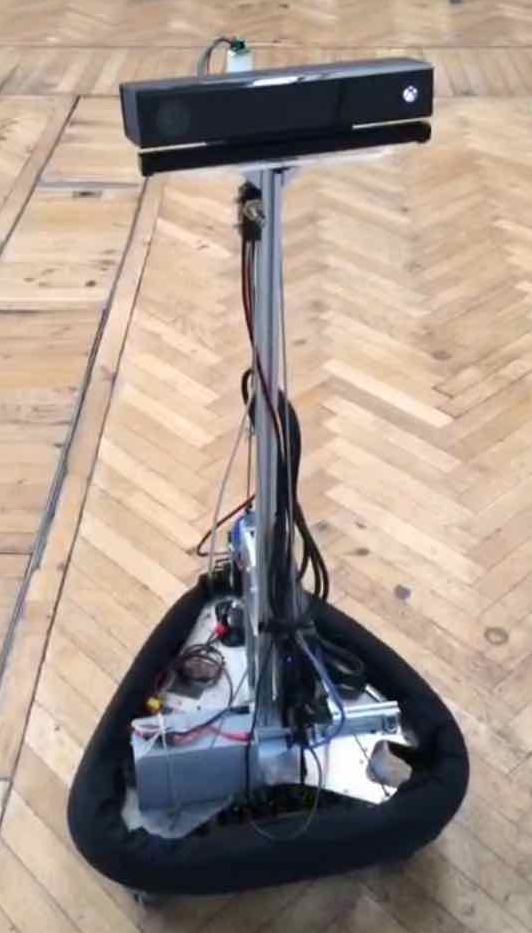
\includegraphics[height=4cm,width=2.5cm]{images/03-foundation/triskar1}}}
	  	\caption{}
	  	\label{fig:evolution_a}
      \end{subfigure}
	 ~
	  \begin{subfigure}[b]{0.22\textwidth}
		\centering
	  	\framebox{\parbox{2.5cm}{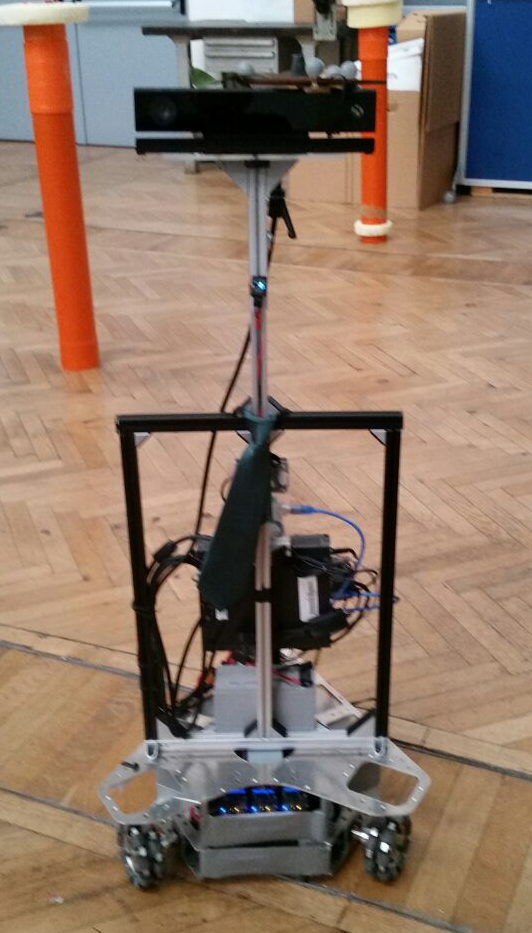
\includegraphics[height=4cm,width=2.5cm]{images/03-foundation/triskar2}}}
	  	\caption{}\label{robot}
      \end{subfigure}
      ~
      \begin{subfigure}[b]{0.22\textwidth}
      	\centering
      	\framebox{\parbox{2.5cm}{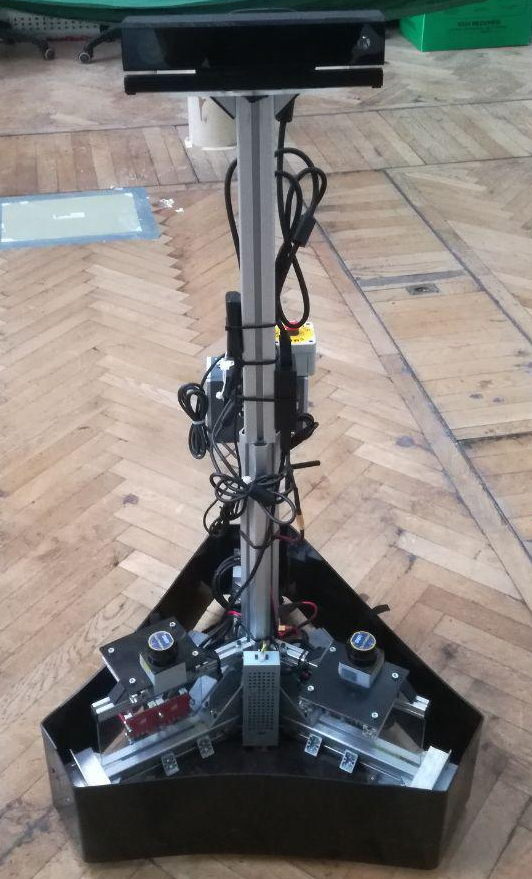
\includegraphics[height=4cm,width=2.5cm]{images/03-foundation/triskar3}}}
      	\caption{}
      \end{subfigure}
      ~
      \begin{subfigure}[b]{0.22\textwidth}
	      \centering
	      \framebox{\parbox{2.5cm}{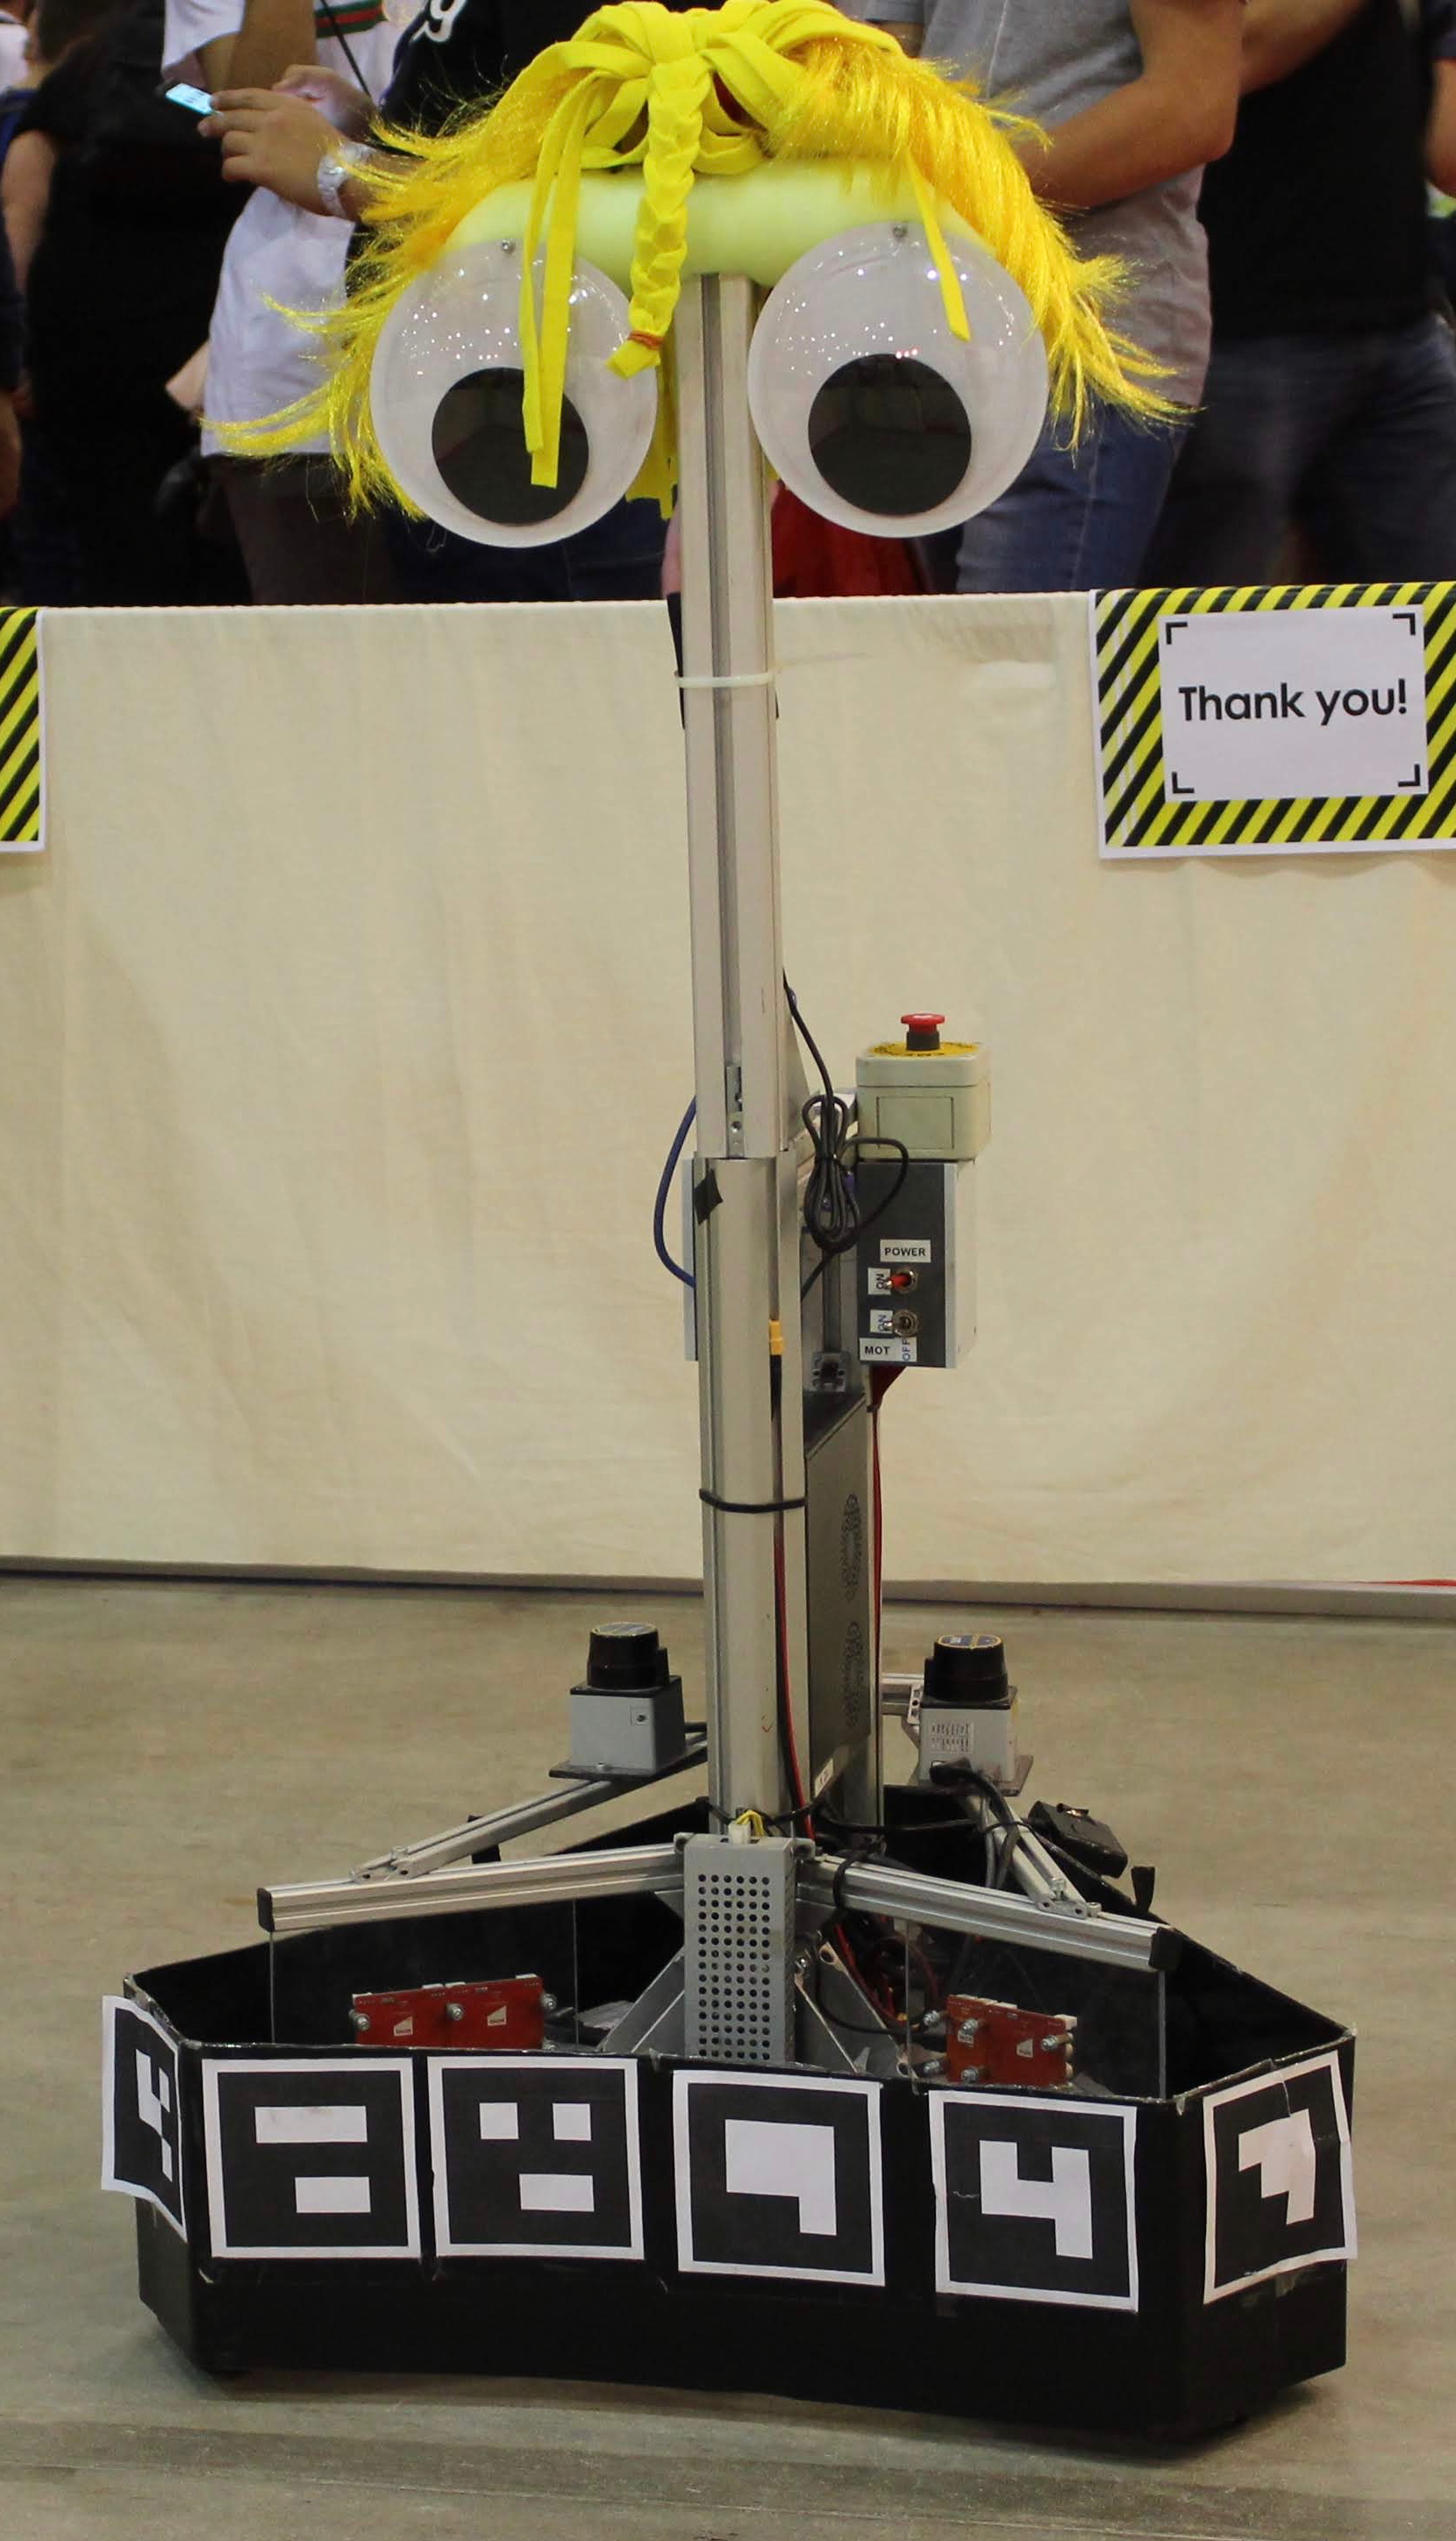
\includegraphics[height=4cm,width=2.5cm]{images/03-foundation/base4.png}}}
	      \caption{}
      \end{subfigure}
      \caption{Prototype evolution. a) First version having the Microsoft Kinect\textsuperscript{\textregistered} camera sensor support secured by steel cables in order to reduce vibration due to motion. b) Second version had improved stability by replacing the steel cables by rigid modular aluminum profiles. c) Third version had a completely redefined base including new electronics, thicker aluminum chassi, redesigned power distribution system and 2D lasers. This version also had a larger base compared to previous prototypes; d) Current version during demonstration at the Maker Faire 2018 in Rome (the European edition) from October 12th to 14th of 2018. A better placement of lasers had made the use of Kinect\textsuperscript{\textregistered} unnecessary since it allowed for full 360\textsuperscript{$\circ$} laser sensing coverage.}
      \label{fig:evolution}
\end{figure}

\subsection{Sensing}
\subsubsection{Microsoft Kinect\textsuperscript{\textregistered}\label{sec:kinectsec}}
In some phases of our development we have used the Microsoft Kinect\textsuperscript{\textregistered} sensor. It is a 3-D camera: in addition to providing an RGB image with its 1080p color camera, it also provides a depth map,  meaning that for every pixel of the depth image provided by the sensor, Kinect\textsuperscript{\textregistered} provides the distance from the sensor (see appendix~\ref{app:hard_appendix} for sensor specifications). 

\subsubsection{Laser scanners}\label{sec:lasers_hokuyo}
We have equipped our robot with two Hokuyo laser scanners model URG-04LX\footnote{\url{https://www.hokuyo-aut.jp/search/single.php?serial=165} accessed on \today.}. The sensors perceive the range of obstacles on a plan with a field of view of 240$^\circ$ and a resolution of 0.36$^\circ$, the maximum detectable distance is 5.6 m and they can be connected to the computer by means of a USB interface, being operated with a nominal voltage of 5V.

A full scan is performed every 100 ms. We mounted a laser scanner on each side of the lower chassis allowing for a 360$^\circ$ coverage around the robot at a height of 30 cm from the floor.

\subsection{Structure \& Materials}
\subsubsection{Chassis}
The chassis of our robot was made entirely from modular aluminum profiles put together as to define the shape in figure~\ref{fig:aluminum_structure} (3rd prototype). The arrangement of the wheels, as to allow for the holonomic behavior, also allowed us to place batteries conveniently~(see figure~\ref{fig:batteries}) as well as the onboard computer and electronics~(see figure~\ref{fig:computer}). The careful placement of heavyweight elements, such as the lead-acid batteries, turned out to be important in our design since it impacted manoeuvrability. For instance, during test it occurred that, due to inertia, the robot would become vertically unstable when making quick turns or rapidly reacting to the human player's presence. 

The constraint of having the Microsoft Kinect\textsuperscript{\textregistered} sitting on top of an aluminum profile, as to allow maximum visibility from the sensor, moved the center of mass upwards making vertical balance worse. The void created between the wheels, in prototype versions three and four, elegantly provided a way to balance weights and make the robot's center of mass close enough to its base center. Figure~\ref{fig:evolution_a} documents the inefficient weight distribution in the first prototype. In the figure its possible to see the placement of one of the lead-acid batteries in the right side of the base, thus, making the weight distribution asymmetric.

Due to forces acting upon the robot during motion we have used software solutions for velocity smoothing that would increasingly bound speed when accelerating and decelerating. This, together with a proper weight distribution, rendered the robot's motion smooth, improving control, at the benefit of reducing the chances of mechanical breakdown caused by material stress.

As an additional way to increase safety, we have considered placing plastic bumpers around the robot so as to reduce potential harms from eventual collision. Despite collisions being rare and negligible in terms of physical harm, the bumpers offered good protection to the electronics. The bumpers can be seen in figure~\ref{fig:evolution}. %TODO This should be put in the HW section. It has nothing to do here. EWERTON: It was in chapter 4, but I move it to here.

\begin{figure}[ht]
    \centering
    \begin{subfigure}[b]{0.22\textwidth}
      	\centering
        \framebox{\parbox{2.5cm}{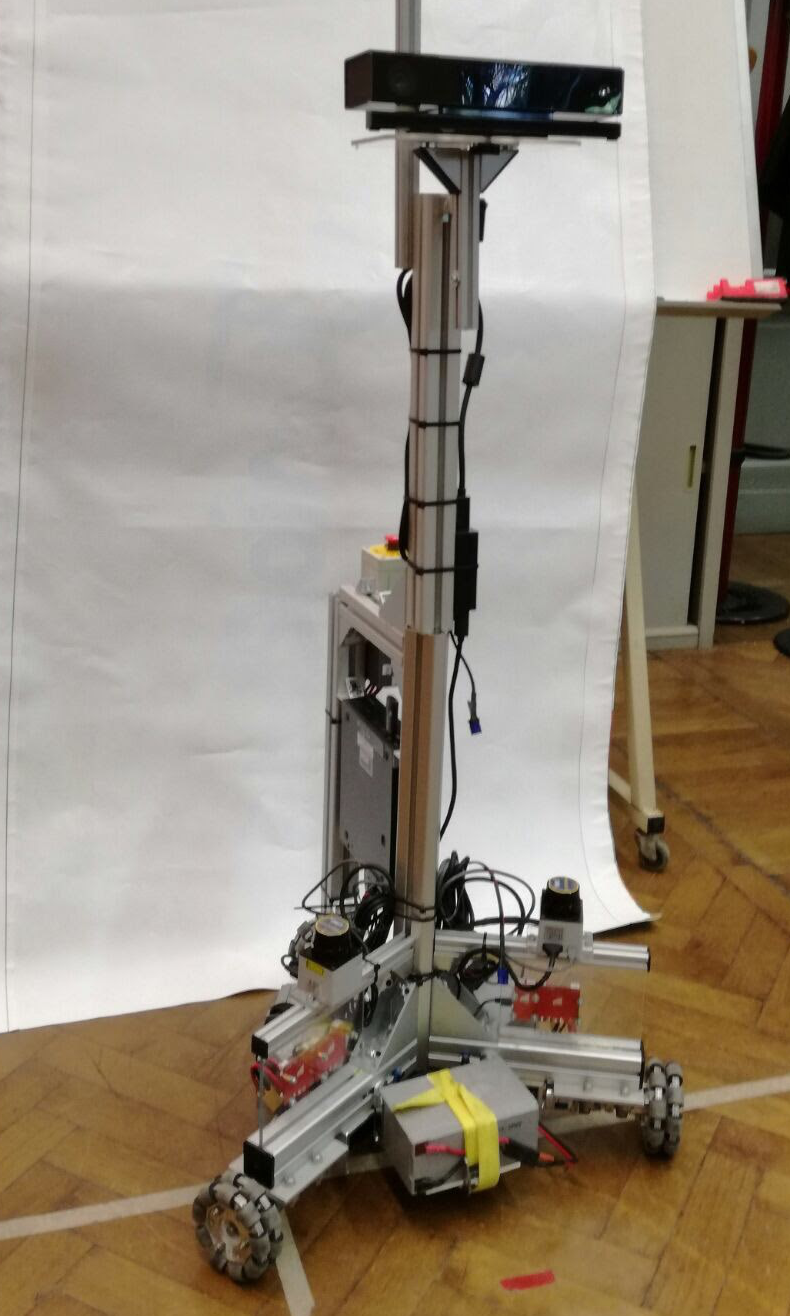
\includegraphics[height=4cm,width=2.5cm]{images/03-foundation/structure}}}
        \caption{}
        \label{fig:aluminum_structure}
    \end{subfigure}
    ~
    \begin{subfigure}[b]{0.22\textwidth}
      	\centering
        \framebox{\parbox{2.5cm}{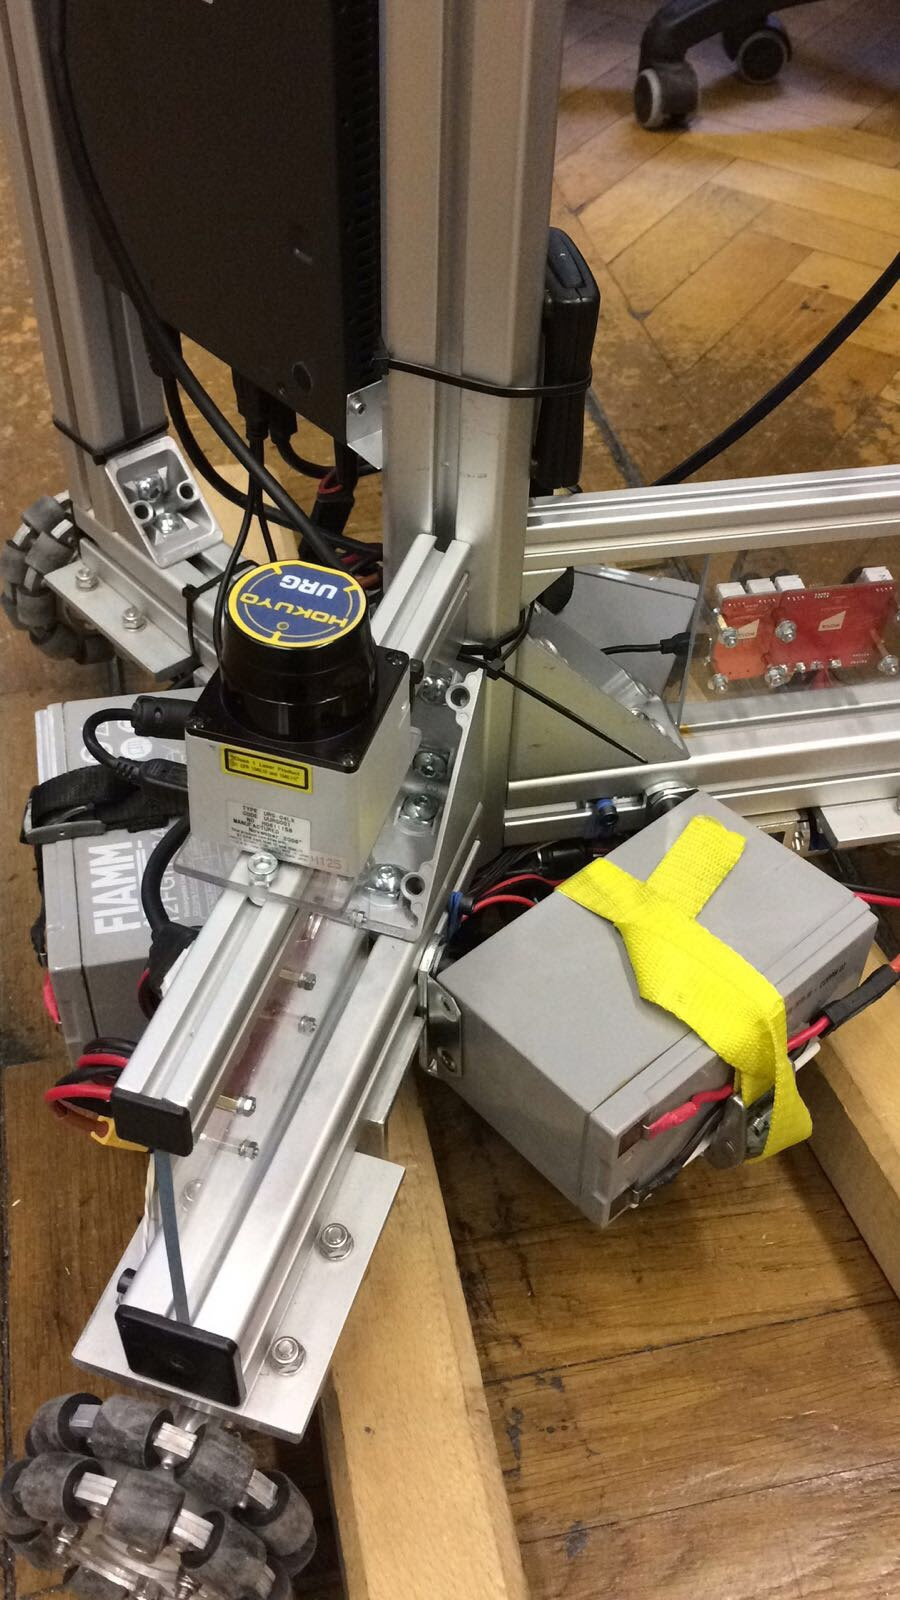
\includegraphics[height=4cm,width=2.5cm]{images/03-foundation/structureII}}}
        \caption{}
        \label{fig:batteries}
    \end{subfigure}
    ~
    \begin{subfigure}[b]{0.22\textwidth}
      	\centering
        \framebox{\parbox{2.5cm}{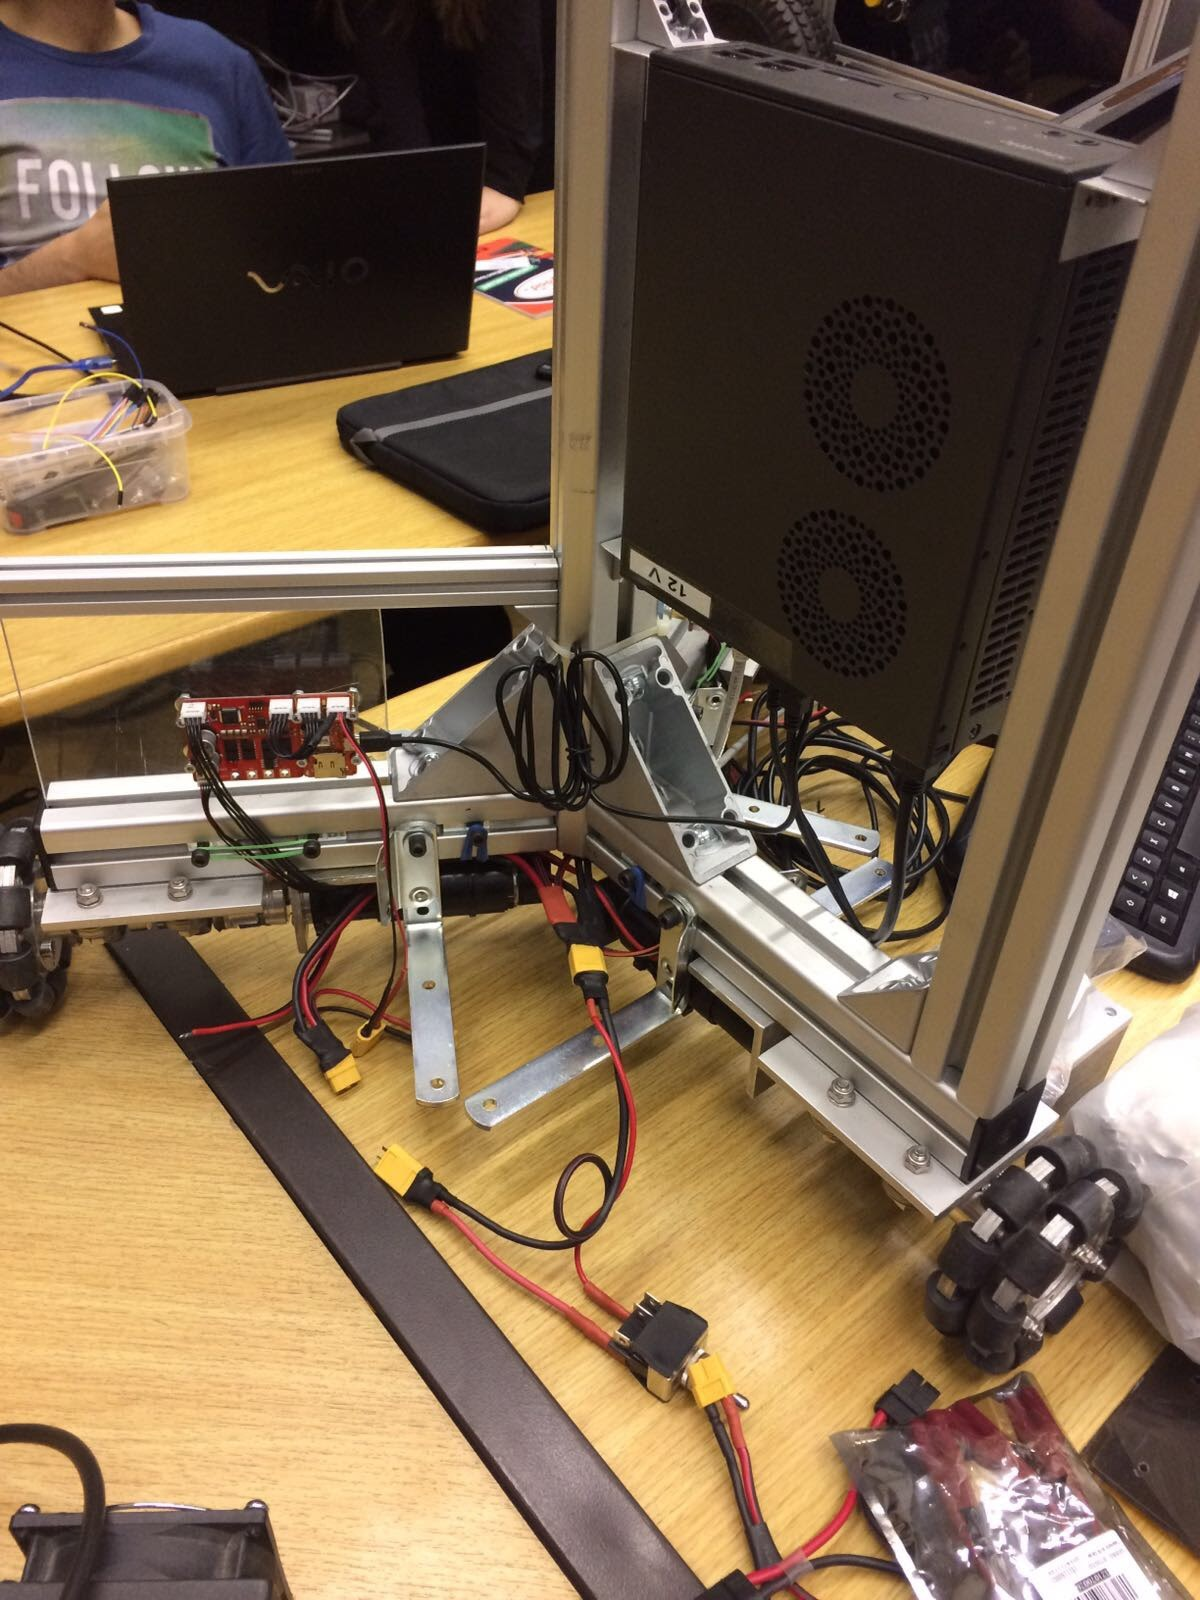
\includegraphics[height=4cm,width=2.5cm]{images/03-foundation/structureIII}}}
        \caption{}
        \label{fig:computer}
    \end{subfigure}
    \caption{Structural details of our robot. The chassis is made of modular aluminum profiles from which rapid and easy prototyping is possible while retaining a good level of robustness. a) The full scale view of the robot (3rd version). b) a close-up view of one of the 2-D lasers and batteries (gray boxes). c) a close-up view of the vertical placement of computer (black box) and control board (red board).}
    \label{fig:structure_details}
\end{figure}

\subsection{Kinematics}
As said before, our robot had holonomic kinematics, i.e. it was capable of moving in any direction in any of the three physical dimensions available to it (i.e., on the floor plan). Our robot matches the kinematics of a human player well, since it is possible to refer to humans as holonomic on the two-dimensional space such as a floor. Mathematical details regarding the kinematics of our 3-wheeled omnidirectional robot is given in appendix~\ref{app:hard_appendix}.


%\subsection{Computing \& Electronics}
%TODO Irrelevant. It would be relevant have an idea of computing power but not even.
%%For computing a Shuttle XPC Slim DH270 was used. The device has a $190 \times 165 \times 43$~mm steel case, and weights $1.3$~kg.  The armature presents two holes for Kensington Locks and numerous threaded holes (M3) at both sides allowing for an easy placement. The operating system used was~\textit{Ubuntu 16.04.3 LTS (64bit)}. The computer had an Intel Core i7 and a RAM DDR4 memory of 16 GB .

%\subsubsection{Control boards}\label{novacore}
%The low-level motors actuation and their interface between the~\gls{ros} system have been realized with the Nova Core modules based on STM32-chip~\footnote{\url{http://www.novalabs.io/} accessed on \today.}, which implement ready to use components to fulfill robot prototyping requirements with plug \& play approach.  
%The provided modules allow to control different type of motors that can be modeled as a second order system, where the input is the voltage applied to the motor armature and output variable is the motor angular speed. Futher details about the deployed boards are presented in figure~\ref{fig:boards}.

%\begin{figure}[ht]
% \centering
%  \begin{subfigure}[b]{0.3\textwidth}
%  \centering
%      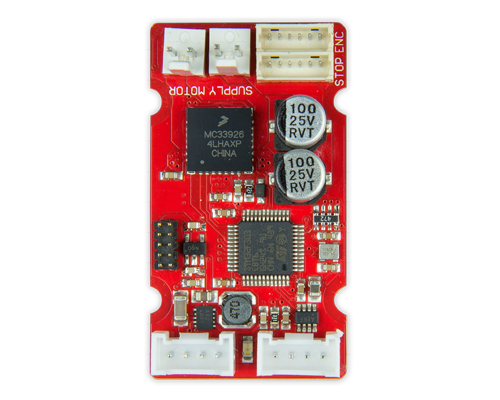
\includegraphics[width=3cm,height=2.5cm]{images/03-foundation/udc}
%	\caption{}
%  \end{subfigure}
%  \begin{subfigure}[b]{0.3\textwidth}
%  \centering
%      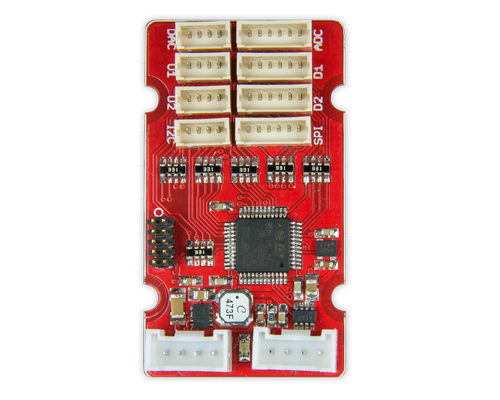
\includegraphics[width=3cm,height=2.5cm]{images/03-foundation/io}
%	\caption{}
%  \end{subfigure}
%  \begin{subfigure}[b]{0.3\textwidth}
%  \centering
%      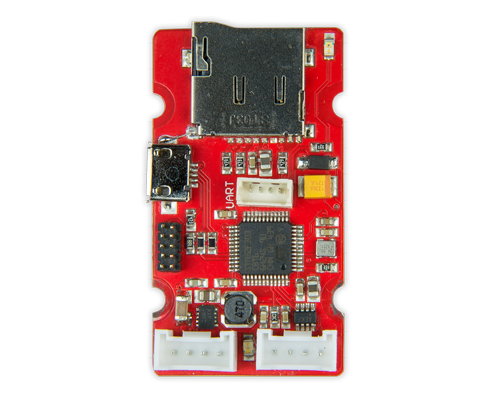
\includegraphics[width=3cm,height=2.5cm]{images/03-foundation/usb}
%	\caption{}
%	\label{fig:usb_board}
%  \end{subfigure}
%  \caption{a) UDC board (1 per each motor) capable of driving motors up to 70 W, with torque, speed, and position closed loop control. General attributes: 5-28V supply; 3A max (5A peak); current sense; encoder input; limit switch input; 25 x 45 mm in size. b) IO board (1 per each motor): Integrate existing hardware into the real-time Nova Core bus with analog and digital signals. General attributes: 8 digital GPIO;  4 analog inputs; 2 analog outputs; 2 UART; 1 I2C; 1 SPI; 25 x 45 mm in size. c) USB board (used for data collection) Interface the real-time Nova Core bus with a computer and logs data to microSD memory. General attributes: USB connector;  UART connector; microSD card slot; rosserial support; 25 x 45 mm in size.}
%  \label{fig:boards}
%\end{figure}

%TODO (still, in part) All the technical details and names of devices could go in an appendix, while I'll leave here a functional description of robot and sensors, giving the characteristics that are functionally relevant, e.g., speed, omnidirectionality, range of sensors, their data rate, ...

\subsection{Navigation}\label{sec:navigation}
\subsubsection{\glsdesc{slam}}\label{gmapping}
To create a map of the environment, our system used \textit{gmapping}\footnote{http://wiki.ros.org/gmapping accessed on \today}, a~\gls{ros} package used for~\gls{slam} that estimates the map of the environment and the trajectory of the robot using a technique known as~\gls{rbpf}~\citep{grisettiyz_improving_2005} and the provided odometry and laser measurements. The procedure in\textit{gmapping} can be decomposed in two phases: \begin{inparaenum}[\itshape a\upshape)]\item update the robot's state using all available positioning related data. In our case, odometry and laser measurements were used; \item update the map of the environment using~\gls{rbpf}.\end{inparaenum}

The obtained map is an occupancy grid and it is represented as an image showing the blueprint of the environment. Once created, the integrated localization in~\gls{ros} will be able to generate reference frame transforms from the map-frame to the robot odometry frame, correcting for estimated position in the environment. In Figure~\ref{fig:playground_map} an example of map is shown, with tower positions being clearly visible.

Considering only the playground (area of the rectangle delimited by four towers), however, introduce several problems to the localization algorithm. For instance, when the playground is put in a rectangular room with only the towers as ``furniture'' the symmetry of the environment does not possess enough descriptive features to infer the position unequivocally and localization is worsened. For this reason it was needed to include enough descriptive features around the playground borders to enhance the robot localization during the game. The map in figure~\ref{fig:playground_map} is a good example of a map with good features since the walls around the playground are ``jagged enough'' to distinguish the walls among themselves. 

\begin{figure}[h]
	\centering
	\framebox{\parbox{5cm}{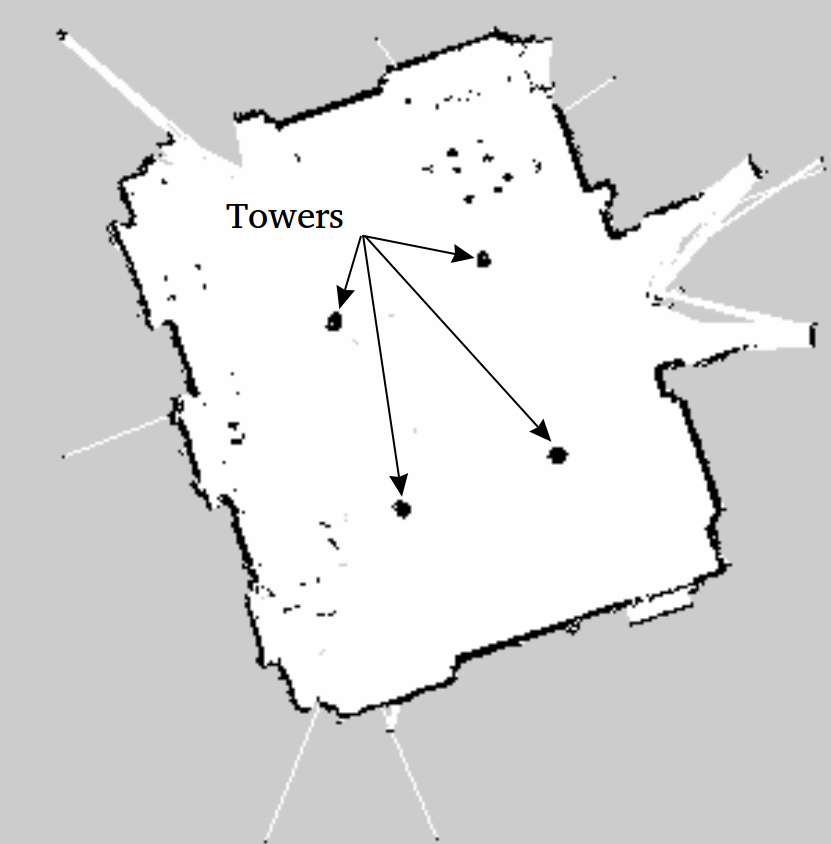
\includegraphics[width=5cm]{images/03-foundation/playgroundmap}}}
	\caption{Map of the room with playground obtained with gmapping algorithm.} 
	\label{fig:playground_map}
\end{figure}

In particular, aiming at standardizing the map across different environments, and at reducing the number of times it had to be remade and filtered out for noise, we have decided to enclose the playground in ``walls'' made from fabric and supported by lightweight aluminum profiles joined together. A custom entrance made in one of the sides made up for the element breaking the symmetry and allowing for effective localization. This arrangement could easily be reused without having to regenerate the map. Enclosing the area was particularly useful when collecting data since very often~\glspl{pirg} tend to gather a number of people around the playground which can compromise the environmental perception by the robot. Furthermore, it allowed us to reduce the complexity of tracking the player, as it is going to be explained in section~\ref{sec:player_tracking}.

\subsection{Basic navigation and control}
In this section we describe the algorithm that enables the robot to navigate from its current position to a target tower and its implementation. For this purpose, a point-to-point trajectory following approach has been considered. The proposed strategy is composed of three main parts: sensor data analysis, obstacle detection and goal seeking. In general, with our navigation we wanted to provide a given level of challenge to the human player while also trying to minimize behaviors that could lead to odometry errors and loss of localization in the map. The selection of the target tower takes into account the proximity relationship between the current position of the robot and that of the human player. The particular algorithm for this is going to be presented later, in section~\ref{sec:competitive_adv_robotower2}.

Generally, the selection of a target tower by the robot is performed so that the direct path leading to it is as free as possible considering the current player position. 
During navigation, in case the human player is detected closer than a certain safety distance from the moving robot, the algorithm switches to the obstacle avoidance procedure described in section~\ref{sec:obt_avoidance}. As inputs to the navigation algorithm, we consider: the robot's estimated $x$ and $y$ position ($\hat{x}_R$, $\hat{y}_R$); target tower xy-coordinate ($x_G$, $y_G$) and a flag variable that assumes the value false if the robot is approaching an obstacle (\verb|is_safe|). The raw outputs are: the unsmoothed xy-linear velocity in the world frame ($\dot{\bar{x}}_R$, $\dot{\bar{y}}_R$) and a flag variable that is true when the robot is close to a targeted tower (\verb|near_goal|). The procedure for generating velocity commands to the platform is detailed in algorithm~\ref{alg:pointopoint}. At each control loop call, the algorithm publishes a new velocity command.

\begin{algorithm}[ht]
	\# define initial e final points when the robot receives the id of the targeted tower \;
	$x_d$ = ($\hat{x}_R$, $x_G$)\;
	$y_d$ = ($\hat{y}_R$, $y_G$)\;
	\# define the robot deviation from the required trajectory\;
	$\Delta x = x_d[1] - x_d[0]$\;
	$\Delta y = y_d[1] - y_d[0]$\;
	\# generates the direction of the motion based on the euclidian distance from goal\;
	goal\_distance$ = \sqrt{({\Delta x}^2 + {\Delta y}^2)}$\;
	$\alpha = $\textbf{atan2}$(\Delta x, \Delta y)$\;
	\# check if the robot is near its goal (this will trigger the obstacle avoidance behavior)\;
	\If{(goal\_distance < NEAR\_GOAL\_Treeshold)}{
		near\_goal = true\;
	}
	\# SAFETY CHECK: the controller will generate velocity commands only if the safety condition is satisfied. if safety condition is satisfied then: enable == 1 (player not too close to the robot);\;
	\If{(is\_safe = true)}{
		$\dot{\bar{x}}_R=V_\text{max}\cdot\cos(\alpha)$\;
		$\dot{\bar{y}}_R=V_\text{max}\cdot\sin(\alpha)$\;
	}
	
	\Return $\dot{\bar{x}}_R$, $\dot{\bar{y}}_R$, is\_safe 
	\caption{Point-to-Point navigation algorithm.}
	\label{alg:pointopoint}
\end{algorithm}

Before being executed by the low-level sub-systems that control the motors, the velocity vector $<\dot{\bar{x}}_R,\dot{\bar{y}}_R>$ produced by algorithm~\ref{alg:pointopoint} need further processing. In particular, it needs to be transformed from the world reference frame (the frame in which towers are located in) to the robot reference frame (see transformation details in appendix~\ref{app:hard_appendix}).

\subsubsection{Slippage control} \label{sec:slippage}
Another aspect to be addressed was about guaranteeing the decoupling between robot rotations and translations. 
This was necessary when using the Kinect\textsuperscript{\textregistered}, since the robot in our scenario had to be able to track the movement of the human player while navigating towards the target towers. Mathematical detail of this process is available in appendix~\ref{app:hard_appendix}. 

Despite all, the transformed velocity set-points $\dot{\bar{x}}_R^m$ and $\dot{\bar{y}}_R^m$, dynamically change during the game and often the variation has a step-function shaped form that causes the low level actuation to react violently to make the robot reach the desired velocity at once -- especially when starting from the initial position with 0-velocity (see figures~\ref{vel14} and~\ref{wheel14}). This will result in the robot wheels undergoing in slippage due to the sharp acceleration required to reach the velocity set-point. This is an undesired effect that is source of non-systematic odometry errors that often lead to instability and loss of localization. 

A number of tests have been performed to quantify the effect of wheel slippage during the initial robot acceleration phase. In these tests the robot linearly translates along $x$ and $y$ axis and receives the initial velocity set-point at $1m/s$ or $1.4m/s$. In figures~\ref{opti14},~\ref{amcl14},~\ref{poserror14},~\ref{opti14y},~\ref{amcl14y}, and~\ref{poserror14y} we can see the localization error introduced during such test.

To avoid this effect, a velocity smoother has been used in order to obtain a smooth velocity set-point control signal to be sent to the robot low-level actuation, in order to avoid wheel slippage during the acceleration phase. The inputs of the velocity smoother are the unsmoothed velocity set-points [$\dot{\bar{x}}_R^m$, $\dot{\bar{y}}_R^m$], some of the internal parameters such as maximum allowed velocity and maximum allowed acceleration can be changed online to modify the final response of the robot. The output are the final xy-velocity control signals [$\dot{x}_R^m$, $\dot{y}_R^m$] in robot reference frame that will be sent to the low level actuation.

The velocity smoother runs together with algorithm~\ref{alg:pointopoint}, receiving the output of this later as input. It basically pre-filters any incoming command input to match some acceleration constraints. Smoothing velocities are not just important for the reduction of localization errors, but is also an important factor in the reduction of material stress on the wheels, which can lead to mechanical breakdowns. In fact, during our research we have had a couple of mechanical breakdown due exactly to excessive acceleration. Such issues make up for important example of typical hardware concerns and issues on must deal with in the design of mobile agents for~\gls{pirg}.

\subsubsection{\glsdesc{oa}}\label{sec:obt_avoidance}
For in-game obstacle avoidance, a fuzzy-logic based reactive control has been designed to respond appropriately to sensory input. This was used principally because the human player could move completely unconstrained in the playground,~\ie proximity between human and robot could be sensed from any direction and in any moment during the game. 

As first step, considering the laser sensing capabilities of our robot (see section~\ref{sec:lasers_hokuyo}), we have divided the rays cast from the laser into different discrete sensing areas around the platform. The information  contained in each laser \verb|\scan| message received from the~\gls{ros} Hokuyo node is composed of 1000 rays, each one of which carrying information about the distance and bearing angle of the sensed object w.r.t the sensor origin. %The laser scan data was divided by indexes as follows: %TODO What these have to do with the fuzzy interpretation reported below? If they are interpreted in a fuzzy way, these intervals have no sense... If two interpretations are superimposed the reader has to understand why and how
% EWERTON: Fuzzy logic had to do with reacting for the player when he is detected in one of the divided zones below. The fuzzy contribution is more important when the player is at the boundaries so as to to allow a smooth reaction. This was reviewed by you in Orrù's thesis. ANDY: Still I cannot understand: either the rays are treated as intervals or as fuzzy sets. What is it done? From below, it seems they are fuzzy sets since there is a fuzzy variable dedicated to this. In this case I would drop this interval-based description. Reading below, and given teh figure I'd drop this

%\begin{itemize}
%	\item \textbf{Rear Right:} indexes from 1 to 150;
%	\item \textbf{Right:} indexes from 151 to 310;
%	\item \textbf{Front Right:} indexes from 311 to 500;
%	\item \textbf{Front Left:} indexes from 501 to 690;
%item \textbf{Left:} indexes from 691 to 851;
%	\item \textbf{Rear Left:} indexes from 850 to 1000.
%\end{itemize}

Having fuzzy-logic rules for the decision making provided soft navigation and stable control since a fuzzy approach can handle well the uncertainty when the sensed obstacle is at the boundary of the sensing areas. 

For each area, the minimum distance to objects are calculated and a flag variable monitors whether an obstacle is within a given threshold distance (in our case 0.75 meters). When this condition is verified, the fuzzy obstacle avoider takes the control from the trajectory navigation in order to handle the obstacle at hand. When the robot is close within a specified distance threshold from a target tower the obstacle avoider is disabled, thus enabling the robot to tear down the towers instead of considering them as obstacles. The output of the avoider is the velocity pair$(V_{x\_\text{avoider}}, V_{y\_ \text{avoider}})$ used to control the xy-translations.

The defined membership functions are shown in figure~\ref{fig:indexesmmf}. On the x-axis are reported the index values in a range from 1 to 1000, each one representing one of the 1000 laser's ray distance measurement that the system receives from each~\gls{ros} \verb|/scan| message.

To interpret the minimum detected distance in each sector the membership functions shown in figure~\ref{fig:minmmf} have been defined. The x-axis ranges from 0 to 0.75 meters (as said, the obstacle avoidance takes control of the robot's navigation when obstacles are detected below this threshold) the three labels ``Close'', ``Far'', and ``Dontcare'' were used to define the intensity of the control action during the obstacle avoidance maneuver.

\begin{figure}[H]
	\centering
	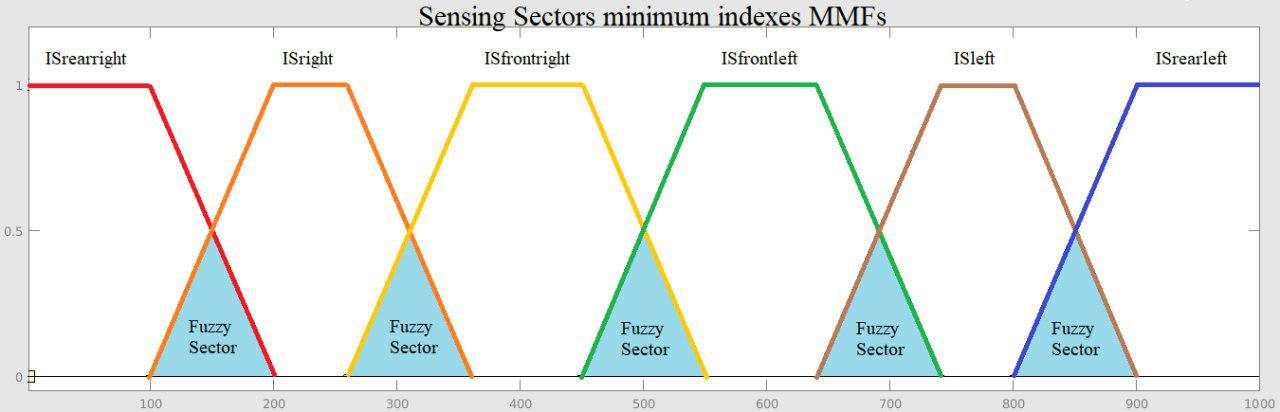
\includegraphics[width=\textwidth]{images/03-foundation/indexesmmf}
	\caption{\glspl{mmf} for the direction of obstacles.} 
	\label{fig:indexesmmf} 
\end{figure}
\begin{figure}[H]
	\centering
	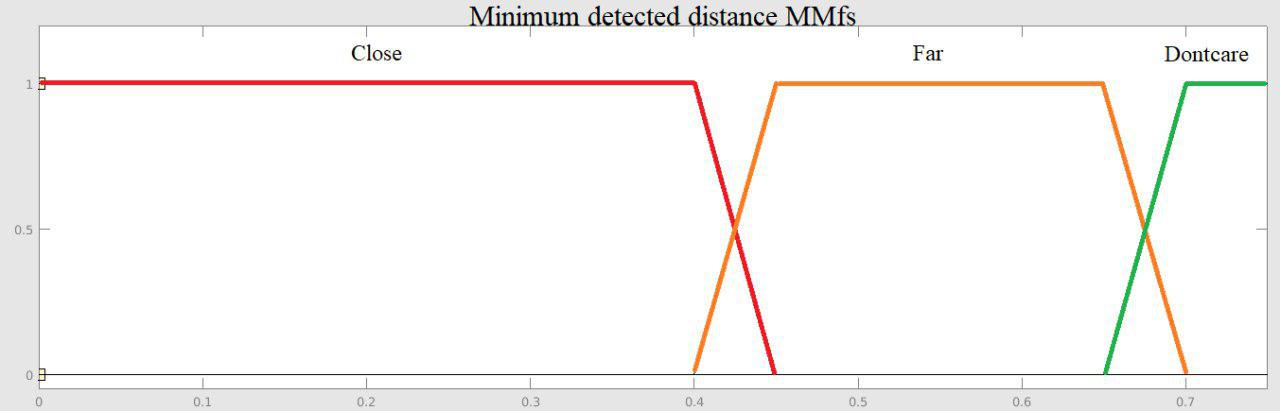
\includegraphics[width=\textwidth]{images/03-foundation/minmmf}
	\caption{\glspl{mmf} for classifying the distance of objects.}
	\label{fig:minmmf} 
\end{figure}

The system uses a Mamdani-type inference that requires the output membership functions to be fuzzy sets. After the aggregation process, \ie after evaluating the result of each rule, these results are combined to obtain a final fuzzy set for each output variable that needs defuzzification.

The selected defuzzification method was the ``Centroid'' method, which returns the center of mass of the area under the resulting fuzzy set membership function, it can also be seen as a Center of Gravity and can be obtained with equation~\ref{centroid}:
\begin{equation}
U=\dfrac{\int_{\text{min}}^{\text{max}} u\cdot\mu(u) du}{\int_{\text{min}}^{\text{max}}\mu(u) du}
\label{centroid}
\end{equation}
where U is the center of gravity, $u$ is the output variable and $\mu(u)$ is the membership function after the accumulation, implemented as the maximum. Letting $\mu_A(u)$ and $\mu_B(u)$ be the membership functions for fuzzy sets A and B and for OR and AND operators are max and min, respectively.
\begin{align}
	\textbf{Accumulation method}\qquad max\lbrace\mu_A(u),\mu_B(u)\rbrace\\
	\textbf{OR (union)}\qquad max\lbrace\mu_A(u),\mu_B(u)\rbrace\\
	\textbf{AND (intersection)}\qquad min\lbrace\mu_A(u),\mu_B(u)\rbrace
\end{align}
As output membership functions, singletons have been selected. This enhances the efficiency of the defuzzification process because it greatly simplifies the computation required by the more general Mamdani method, since, instead of finding the centroid of a 2-D function by integrating across the two-dimensional function to find the centroid, the weighted average of a few data points is used as shown in equation~\ref{singletoncentroid}, where $p$ is the number of singletons.

\begin{equation}
U =	\dfrac{\sum_{i=1}^{p}\left[u_i,\mu_i\right]}{\sum_{i=1}^{p}\mu_i}
\label{singletoncentroid}
\end{equation} 

The singletons membership functions for $V_{x\_ \text{avoider}}$ and $V_{y\_ \text{avoider}}$ are reported in figure \ref{outmmf}

\begin{figure}[h]
	\centering
	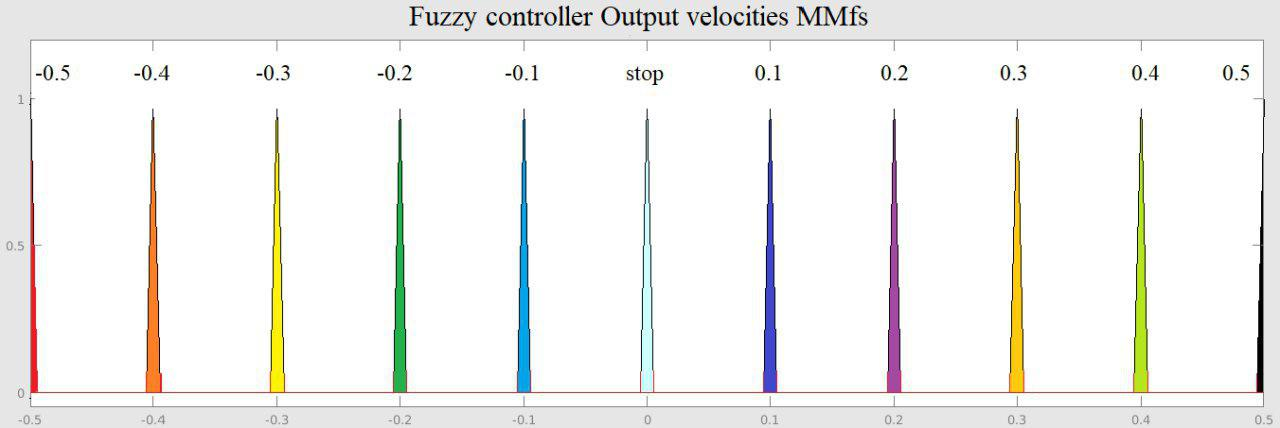
\includegraphics[width=\textwidth]{images/03-foundation/outputmmf}
	\caption{MMfs for $V_{x\_ \text{avoider}}$ and $V_{y\_ \text{avoider}}$, the output velocities along xy-axis range from -0.5 m/s to 0.5 m/s}
	\label{outmmf} 
\end{figure}

A set of fuzzy rules (reported in appendix~\ref{app:hard_appendix})	has been implemented to obtain an overall obstacle avoidance behavior that has been inspired from the artificial potential fields approach. The rules have been designed to mimic a repulsive field that will drive the robot away from obstacles when these are encountered during navigation (figure~\ref{fig:avoid1}). In particular, when the robot reaches the condition of proximity with the human player during the game, the set of fuzzy rules will cause the robot to drift away from him until the proximity condition is no more verified (\verb|is_safe| equals true. Refer to algorithm~\ref{alg:pointopoint}). At this point, the robot will go back to the normal point-to-point navigation to reach the selected target tower.

For the towers, the algorithm defines an attractive effect (figure~\ref{fig:avoid2}) for obstacle estimated to be at the tower positions, which, thus, make it possible to tear down the towers. This is triggered when the robot comes close to the tower positions (\verb|near_goal == true|, again refer to algorithm~\ref{alg:pointopoint}). %TODO It is not clear how this last matches the description of the navigation given before that seemed to bring the robot to the tower. Maybe you may say there that if the obstacle is a tower, the fuzzy algorithm will bring the robot against it, so that when the reader comes here can get no surprise.
% EWERTON: Done.

\begin{figure}[H]
	\centering
	\begin{subfigure}[b]{0.4\textwidth}
		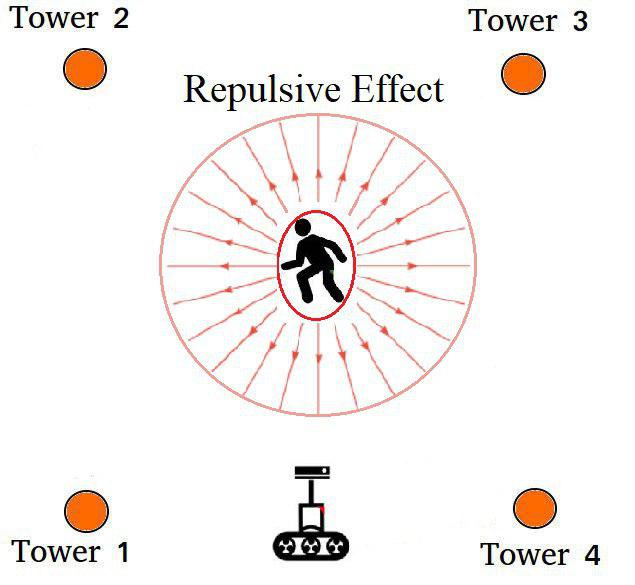
\includegraphics[width=5cm]{images/03-foundation/avoid1}
		\caption{}
		\label{fig:avoid1} 
	\end{subfigure}
    ~
	\begin{subfigure}[b]{0.4\textwidth}
		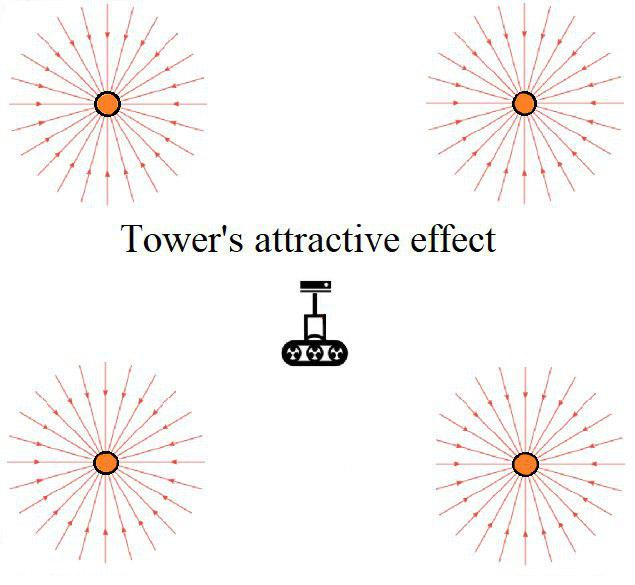
\includegraphics[width=5cm]{images/03-foundation/avoid2}
		\caption{}
		\label{fig:avoid2}
	\end{subfigure}
	\caption{a) Representation of the repulsive effect implemented by the fuzzy rules. b) Representation of the attractive effect implemented by the fuzzy rules. }
	\label{rulesbehavior}
\end{figure}

\subsection{Player perception \& tracking}\label{sec:player_tracking}
In our research we have implement some strategies for player tracking. For the first prototypes, as said before, we have worked with the Kinect\textsuperscript{\textregistered}. %For opening the device, we have used libfreenect2\footnote{~\url{https://github.com/OpenKinect/libfreenect2} accessed on \today.} on Linux.
We have then created a custom tracking node capable of estimating the player's position in two phases: First, by running color blob detection on the RGB image frame. Secondly, by segmenting the player in the depth frame using \textit{region growing} algorithm. The seed for this algorithm is is the position of the blob detected in the first phase.

Two features could be extracted from the procedure: distance (relative to the robot) and contraction index. The first is calculated taking the mean value of the depth pixels around the center of the detected color blob. The latter is computed based on the subtraction of the occupied area with respect to the dimension of the bounding box that encompasses the segmented silhouette (see figure~\ref{fig:segmenta}). The contraction index was intended as a cue about the fact that the player was opening arms, so, possibly, actively participating in the game.

\begin{figure}[h]
  \centering 
  \begin{subfigure}[b]{0.3\textwidth}
		\centering
		\framebox{\parbox{3cm}{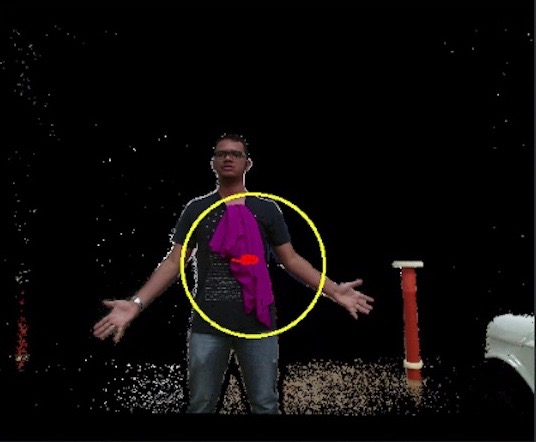
\includegraphics[width=3cm, height=3cm]{images/03-foundation/point_cloud}}}
		\caption{}
  \end{subfigure}
  ~
  \begin{subfigure}[b]{0.3\textwidth}
		\centering
		\framebox{\parbox{3cm}{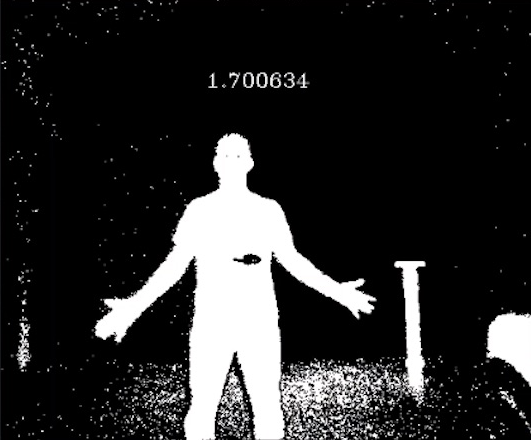
\includegraphics[width=3cm, height=3cm]{images/03-foundation/depth}}}
		\caption{}
  \end{subfigure}
  ~
  \begin{subfigure}[b]{0.3\textwidth}
		\centering
		\framebox{\parbox{3cm}{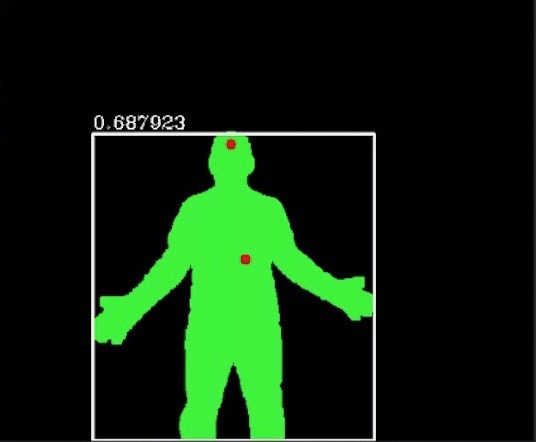
\includegraphics[width=3cm, height=3cm]{images/03-foundation/segmentation}}}
		\caption{}
  \end{subfigure}
  \caption{Example of frames processed by our algorithm. a) Point cloud showing the center of the detected (light-purple) color blob. b) Depth frame. The number showed above the user correspond to his estimated distance relative to the robot (in meters). c) Segmentation results. The number above is the contraction index defined in the interval [0,1] and can be used as a measure of body contraction.}\label{fig:segmenta}
   \label{segmentacao}
\end{figure}

Despite being an useful sensor, its usage in our platform had some issues. One of such was the indirect negative impact in the robot localization caused by having the sensor in a fixed position (see figure~\ref{fig:evolution}). It occurred in our game that the player would run from any side, thus, forcing the tracking algorithms to issue in-place rotation commands to the platform in order to reacquire the player position when he goes out of the~\gls{fov}. Repeatedly rotating the platform in our environment was likely to introduce higher amount of odometry error which contributed to the lack of precision in localization, affecting the accuracy of the platform in navigating toward target towers. Figure~\ref{fig:maps} give an idea of the problem. It is possible to see a higher mismatch between the laser scan and the map of the environment in the subfigure~\ref{fig:laser_map_mismatch} which, in our context, was a consequence of repeatedly rotating the robot in order to keep the player in the~\gls{fov}. 

Other than the localization issues which made the navigation inaccurate (sometimes missing the towers), the need to rotate the player so to keep it in the camera's~\gls{fov} made the interaction slow and, in some cases, clumsy. As a solution to the problem we have later replaced the Kinect\textsuperscript{\textregistered} sensor by a pair of lasers sensors such that a~\gls{fov} of 360$^\circ$ could be granted.

\begin{figure}
    \centering 
    \begin{subfigure}[h]{0.49\columnwidth}
        \centering 
        \framebox{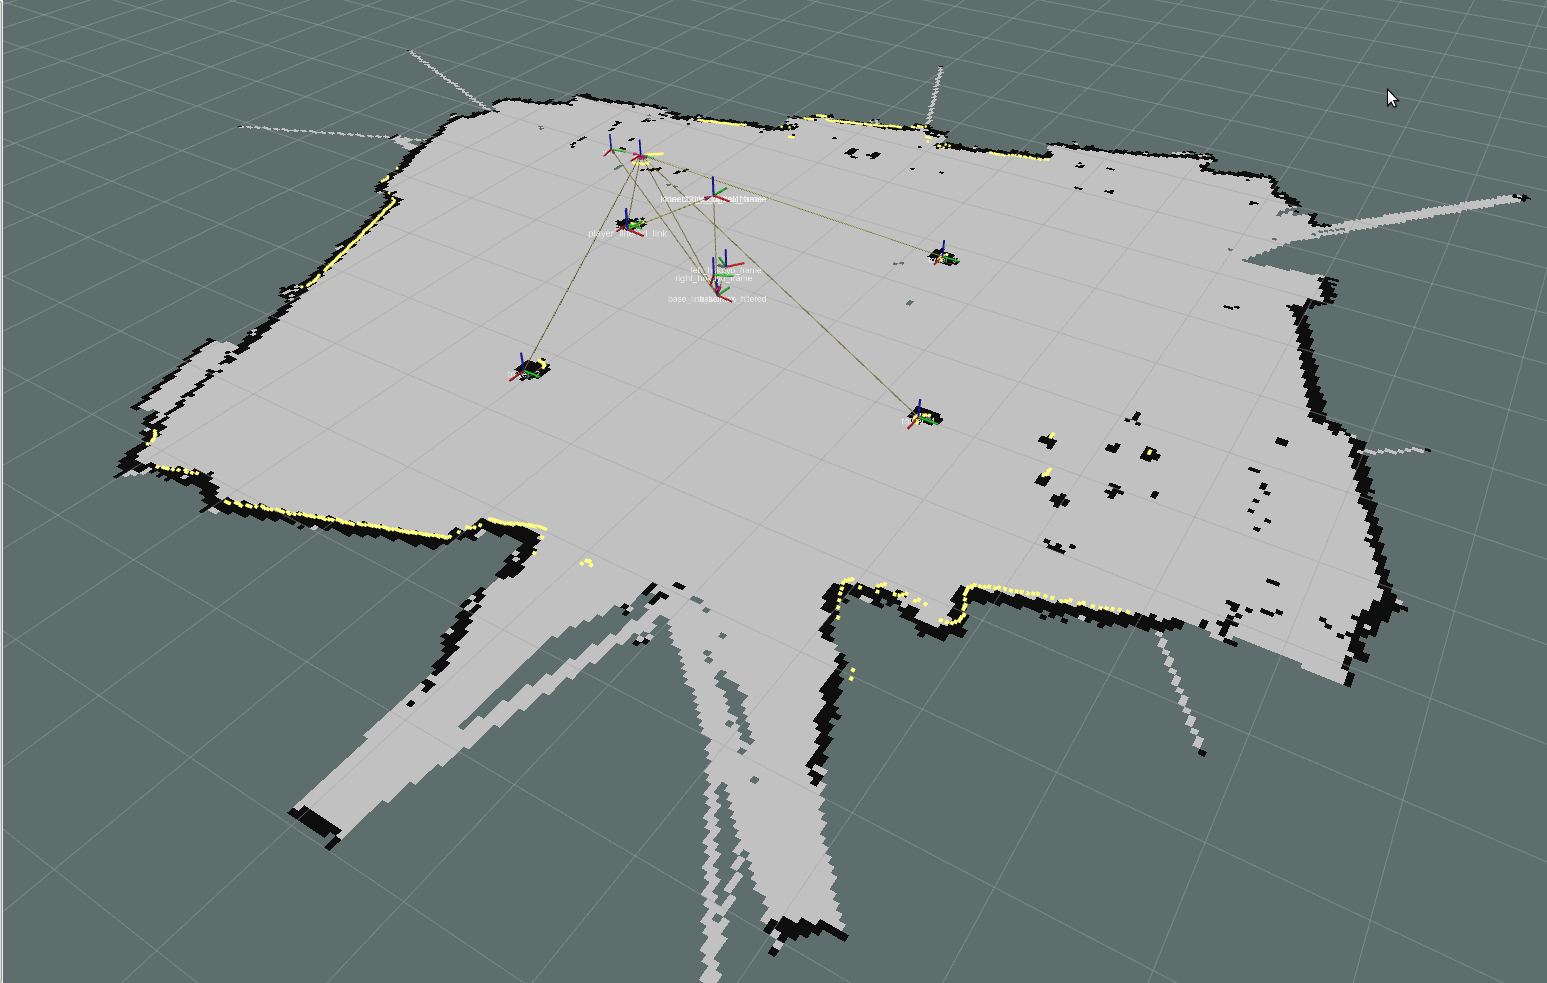
\includegraphics[width=0.95\linewidth]{images/03-foundation/map}}
        \caption{}
    \end{subfigure}
    ~
    \begin{subfigure}[h]{0.49\columnwidth}
        \centering 
        \framebox{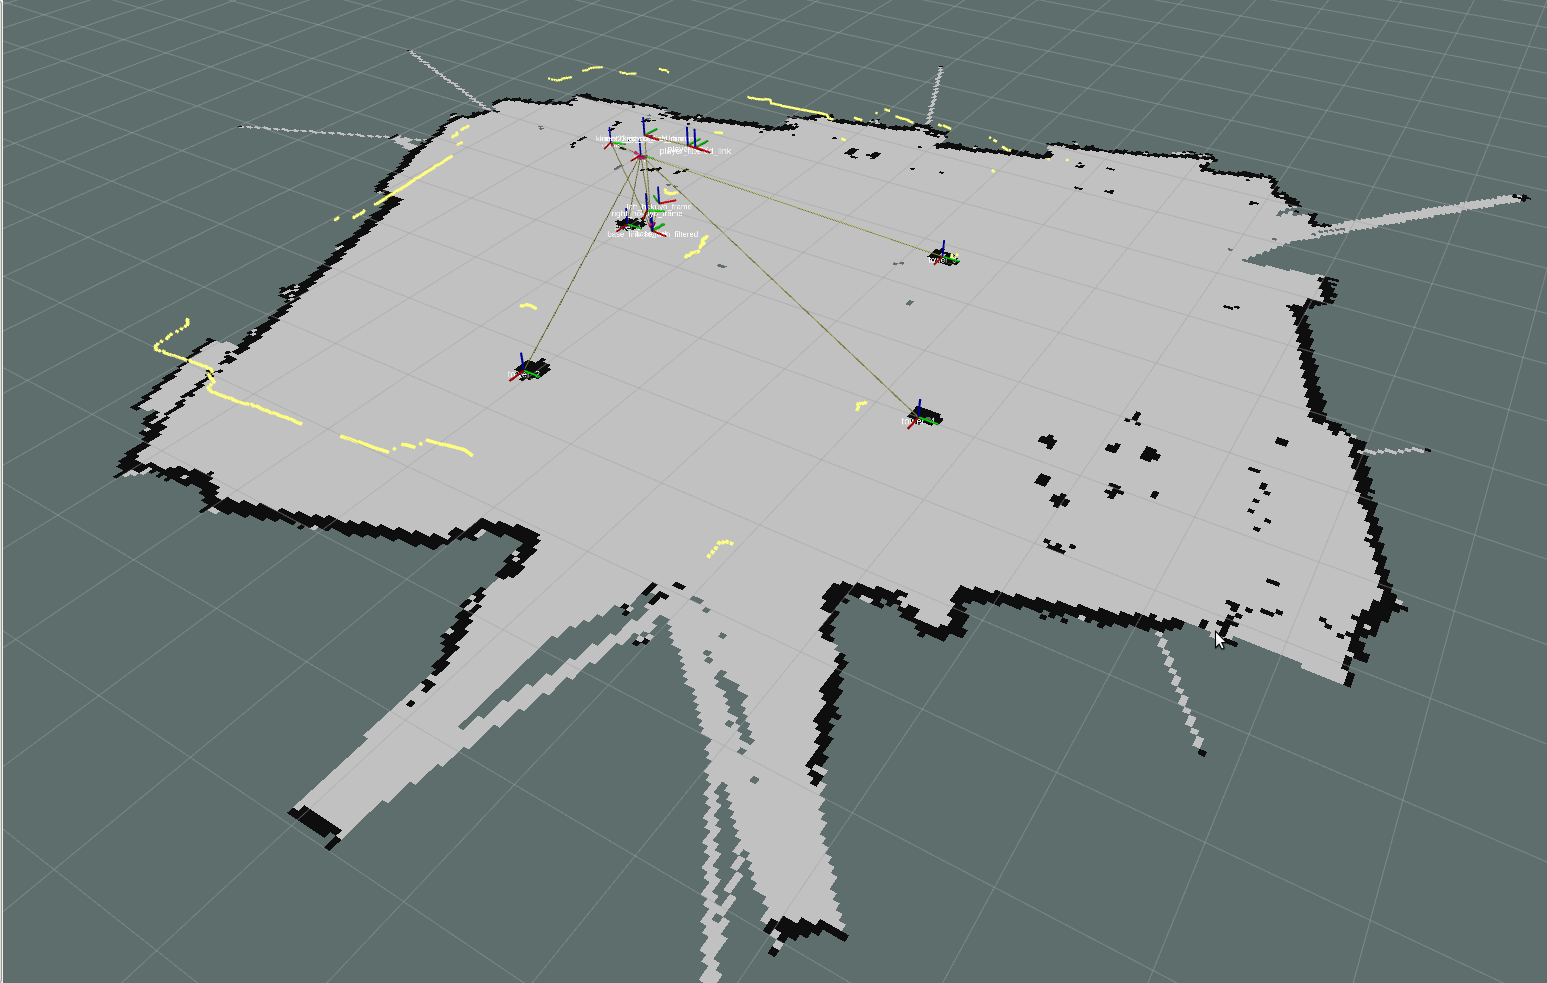
\includegraphics[width=0.95\linewidth]{images/03-foundation/map2}}
        \caption{}
        \label{fig:laser_map_mismatch}
    \end{subfigure}
    \caption{a) Example of good localization. b) Example of low-quality localization where the laser scan (yellow traces) mismatch with the map of the room.}
    \label{fig:maps}
\end{figure}

The \textcolor{red}{...}